\input{../header}
\usepackage{pgfplots}
\rhead{Your name: \rule{8cm}{0.15mm}}

\begin{document}

\section{Learning target DFb, version 1}

Given a graph of a function, estimate specific values of the derivative, and/or produce a sketch of the derivative function.

\hrulefill

Here is the graph of some wacky function $q(x)$:

\begin{center}
    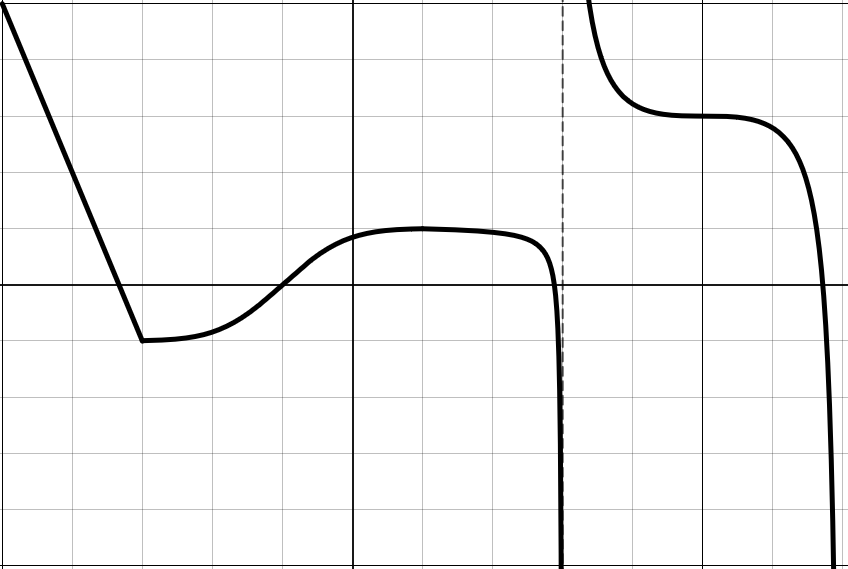
\includegraphics[width=0.85\textwidth]{../images/DFb-v1.png}    
\end{center}


Sketch the graph of $q'(x)$ on the blank axes below.

\begin{center}
    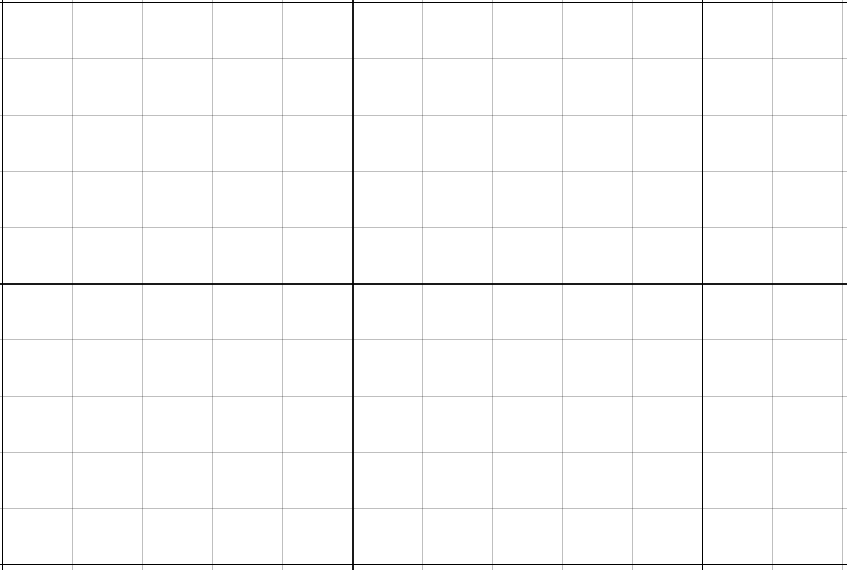
\includegraphics[width=0.85\textwidth]{../images/DFb-v1-blank.png}    
\end{center}

%%%%%%%%%%%%%%%%%%%%%%%%%%%%%%%%%%%%%%%%%%%%%%%%%%%%%%%%%
\pagebreak
%%%%%%%%%%%%%%%%%%%%%%%%%%%%%%%%%%%%%%%%%%%%%%%%%%%%%%%%%

\section{Learning target DFb, version 2}

Given a graph of a function, estimate specific values of the derivative, and/or produce a sketch of the derivative function.

\hrulefill

Here is the graph of some wacky function $h(t)$:

\begin{center}
    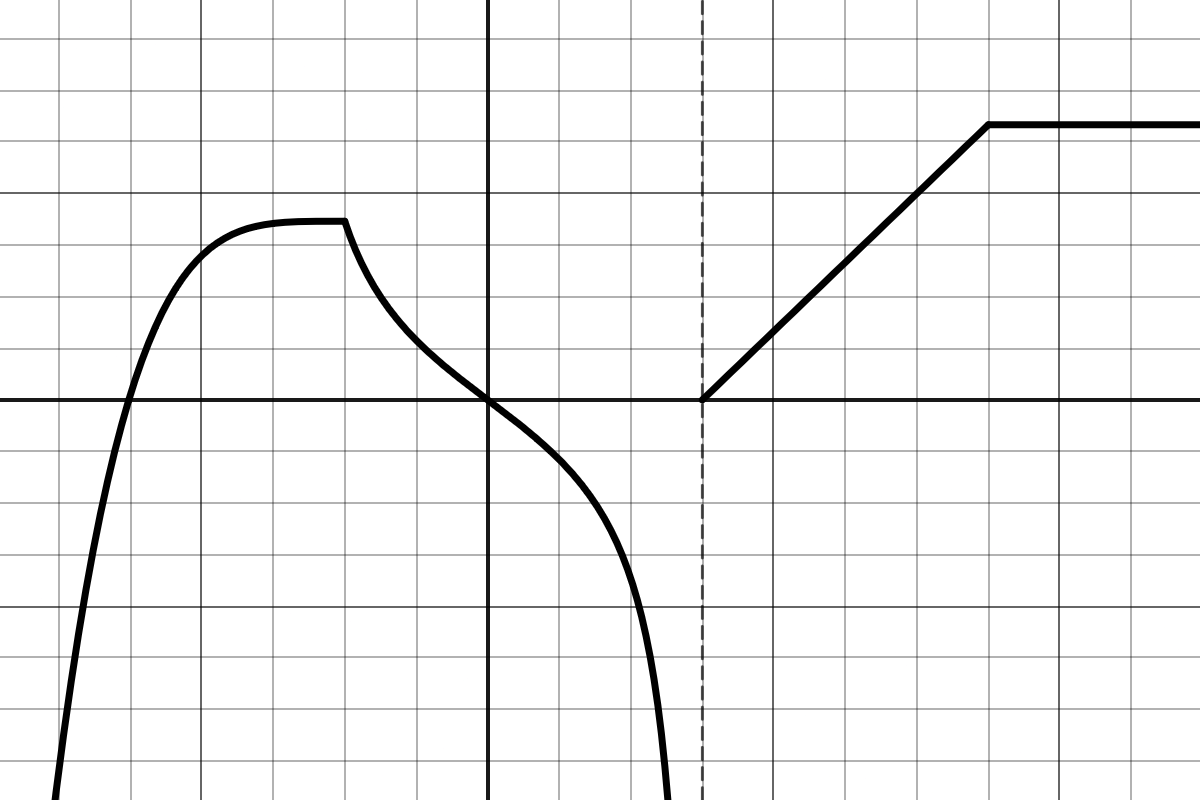
\includegraphics[width=0.85\textwidth]{../images/DFb-v2.png}    
\end{center}


Sketch the graph of $h'(t)$ on the blank axes below.

\begin{center}
    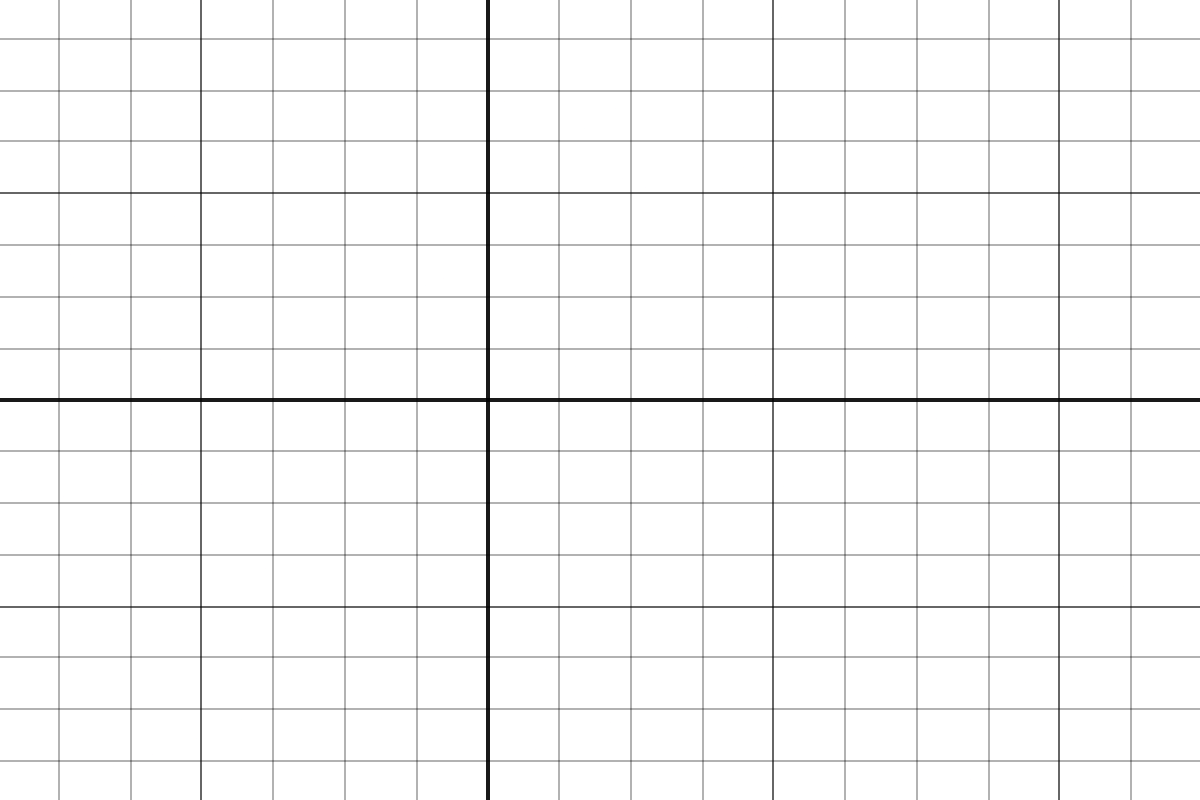
\includegraphics[width=0.85\textwidth]{../images/DFb-v2-blank.png}    
\end{center}

%%%%%%%%%%%%%%%%%%%%%%%%%%%%%%%%%%%%%%%%%%%%%%%%%%%%%%%%%
\pagebreak
%%%%%%%%%%%%%%%%%%%%%%%%%%%%%%%%%%%%%%%%%%%%%%%%%%%%%%%%%
\section{Learning target DFb, version 3}

Given a graph of a function, estimate specific values of the derivative, and/or produce a sketch of the derivative function.

\hrulefill

Here is the graph of some wacky function $z(x)$:

\begin{center}
    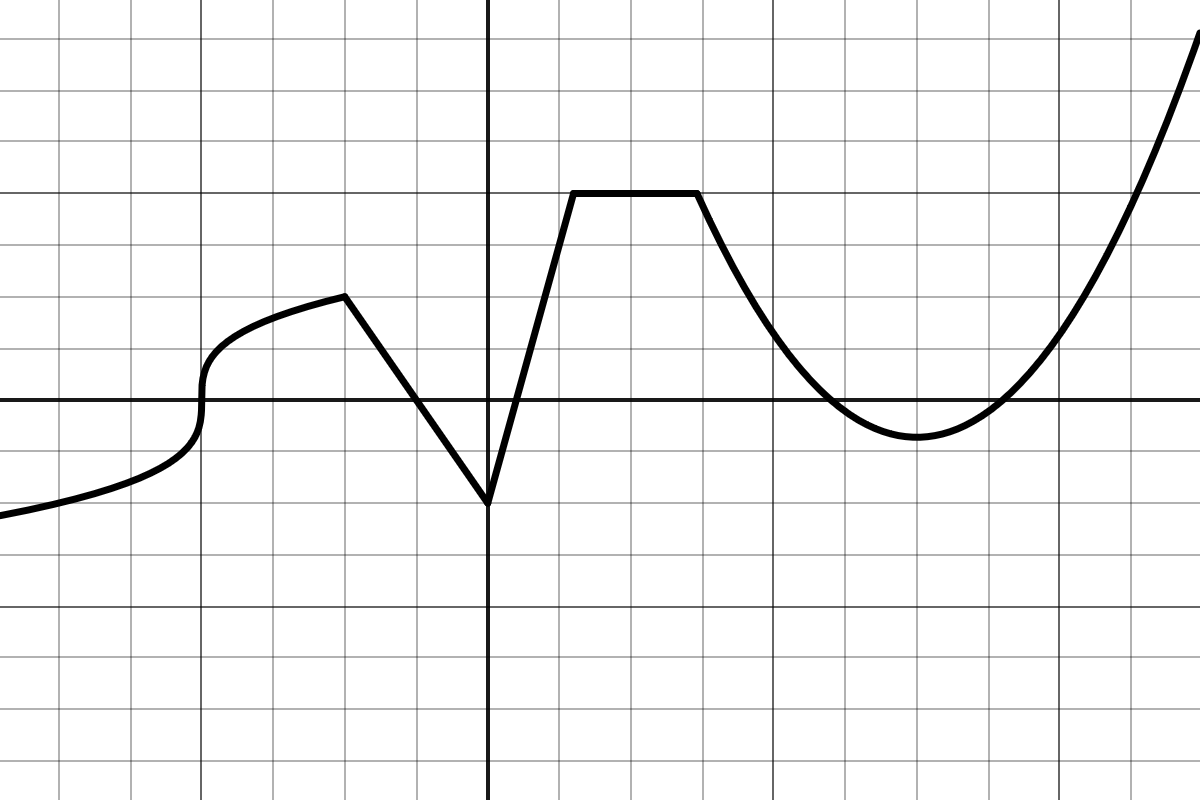
\includegraphics[width=0.85\textwidth]{../images/DFb-v3.png}    
\end{center}


Sketch the graph of $z'(x)$ on the blank axes below.

\begin{center}
    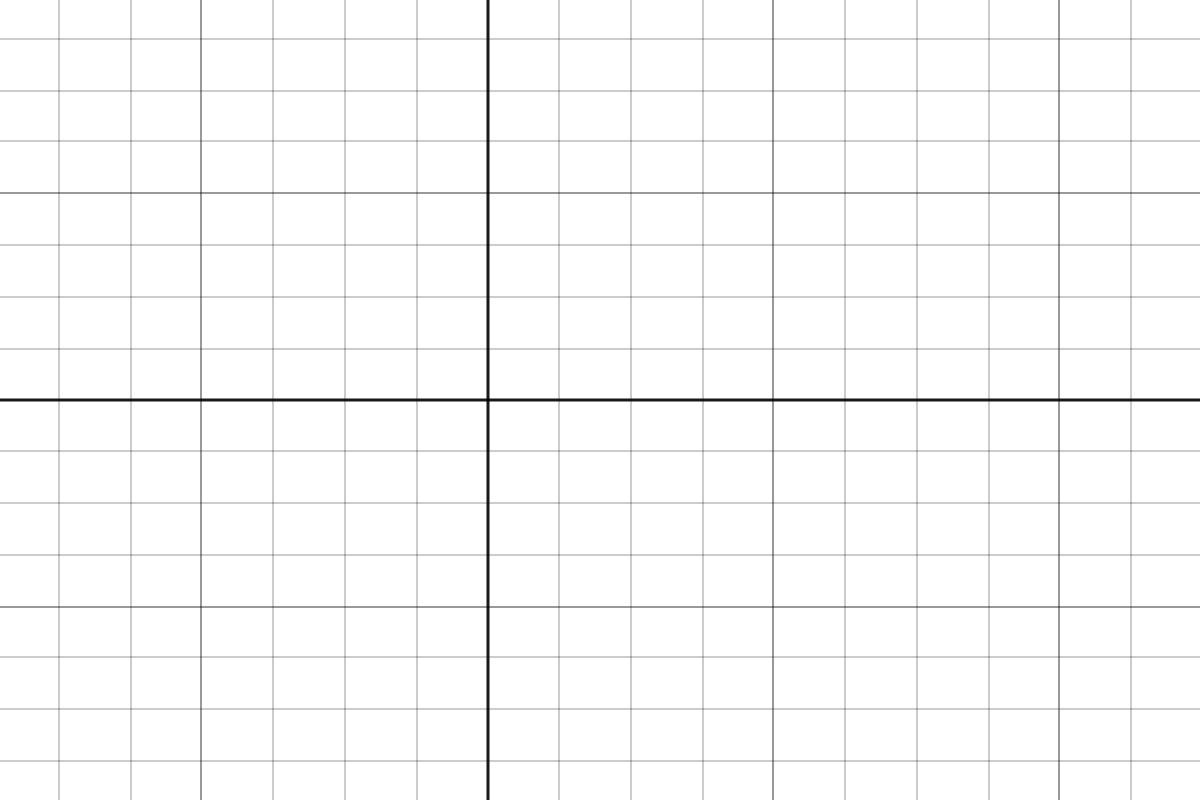
\includegraphics[width=0.85\textwidth]{../images/DFb-v3-blank.png}    
\end{center}

%%%%%%%%%%%%%%%%%%%%%%%%%%%%%%%%%%%%%%%%%%%%%%%%%%%%%%%%%
\pagebreak
%%%%%%%%%%%%%%%%%%%%%%%%%%%%%%%%%%%%%%%%%%%%%%%%%%%%%%%%%
\section{Learning target DFb, version 4}

Given a graph of a function, estimate specific values of the derivative, and/or produce a sketch of the derivative function.

\hrulefill

Here is the graph of some wacky function $g(t)$:

\begin{center}
    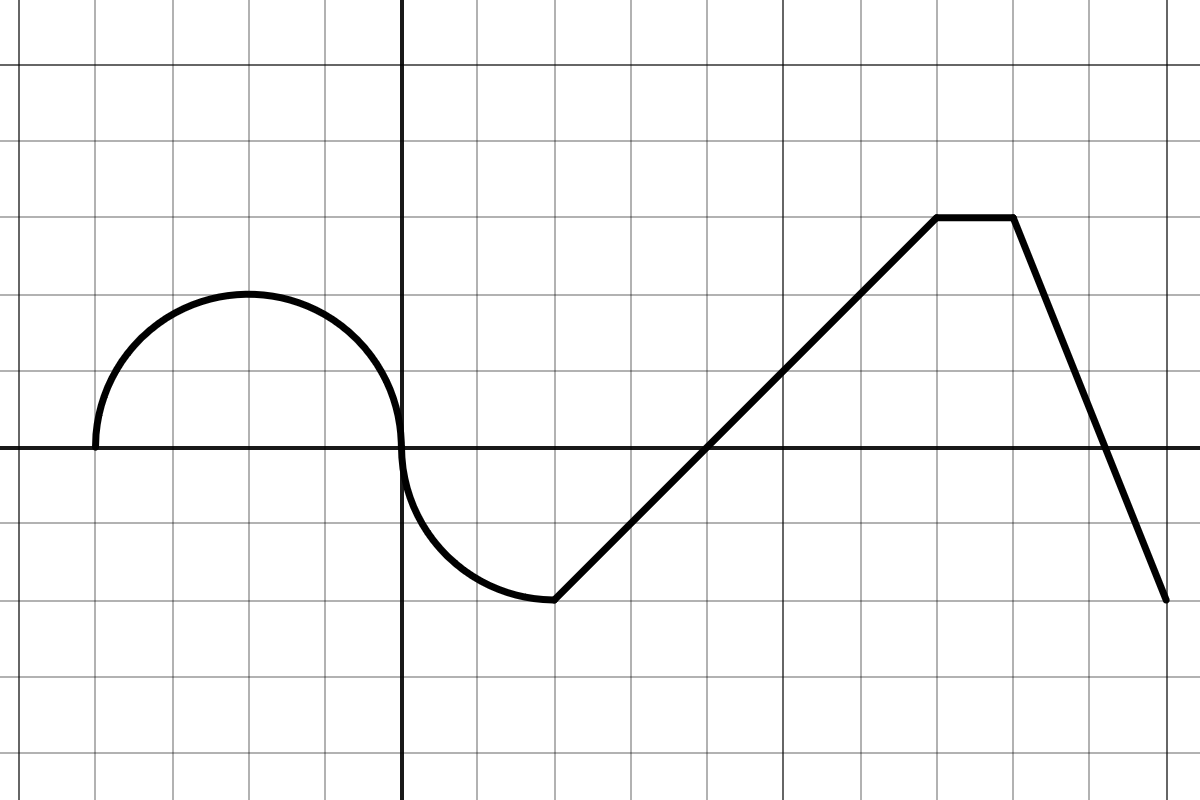
\includegraphics[width=0.85\textwidth]{../images/DFb-v4.png}    
\end{center}


Sketch the graph of $g'(t)$ on the blank axes below.

\begin{center}
    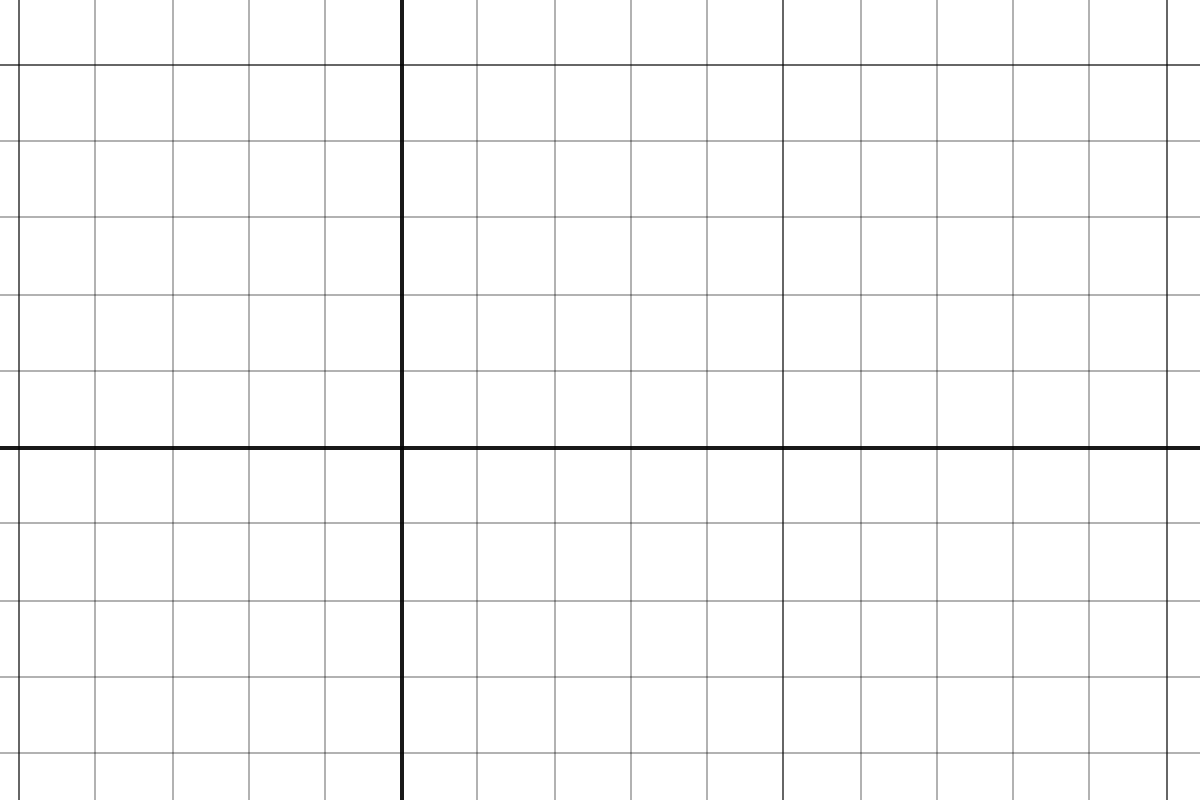
\includegraphics[width=0.85\textwidth]{../images/DFb-v4-blank.png}    
\end{center}

%%%%%%%%%%%%%%%%%%%%%%%%%%%%%%%%%%%%%%%%%%%%%%%%%%%%%%%%%
\pagebreak
%%%%%%%%%%%%%%%%%%%%%%%%%%%%%%%%%%%%%%%%%%%%%%%%%%%%%%%%%
\end{document}